% Agregar:
% antecedentes recolectados
% otros (imágenes, textos, tablas, etc.)




\subsection{Actividades y tiempos empleados por cada integrante}

\begin{tabular}{|l|p{7cm}|c|}
\hline
Integrante & Actividades & Tiempo Empleado \\\hline
Cristián Maureira & Observación de los medios de comunicación y reuniones internacionales. & 7 horas \\
& Creación del Repositorio de trabajo. & 30 minutos \\
& Creación del esqueleto del informe.& 30 minutos \\
& Desarrollo de la introducción. & 2.5 horas \\
& Redacción de los análisis y resultados de antecedentes. & 3 horas \\
& Revisión de los análisis y resultados de antecedentes. & 1 hora \\
\hline
Gabriel Zamora & Revisión de  las formas de trabajo de cada grupo. & 8 horas \\
& Estudio del público objetivo y del dominio del trabajo. & 3 horas \\
& Redacción de los análisis y resultados de antecedentes. & 4 horas \\
\hline
Rodrigo Fernández & Comparación de los resultados con los antecedentes
recopilados. & 5 horas \\
& Investigación de la información existente. & 5 horas \\
& Redacción de los análisis y resultados de antecedentes. & 3 horas \\
& Revisión del análisis y resultados de antecedentes. & 30 minutos \\
& Revisión ortográfica del informe. & 10 minutos \\
\hline
\end{tabular}
\newpage
\subsection{Participantes de las reuniones}
\subsubsection{OSF Coordination Meeting}

\begin{tabular}{|l|l|l|l|}
	\hline
	{\bf Nombre} & {\bf Cargo} & {\bf Organización} & {\bf País} \\\hline
	Heiko Sommers & ACS Technical Leader & ESO & Alemania \\\hline
	Gianluca Chiozzi & ESO Astronomical Instrumentation Leader & ESO & Italia \\\hline
	Alessandro Caproni & Software Engineer& ESO & Italia \\\hline
	Matias Mora & Software Engineer & ALMA & Chile \\\hline
	Nicolas Troncoso & Software Engineer & ALMA & Chile \\\hline
	Jorge Avarias & Software Engineer & NRAO & EEUU \\\hline
	Rodrigo Tobar & Software Engineer & ESO & Alemania \\\hline
	Jaime Pavlich & Profesor & UCN & Chile \\\hline
	Tomas Staig & Computer Science Student & UTFSM/ESO & Chile \\\hline
	Arturo Hoffstadt & Computer Science Engineer & UTFSM/NRAO & Chile \\\hline
	Gabriel Zamora & Computer SCience Student & UTFSM & Chile \\\hline
	Cristián Maureira & Computer SCience Student & UTFSM & Chile \\\hline	
\end{tabular}

\subsubsection{ACS Weekly Meeting}

\begin{tabular}{|l|l|l|l|}
	\hline
	{\bf Nombre} & {\bf Cargo} & {\bf Organización} & {\bf País} \\\hline
	Joseph Schwarz & ACS Project Leader & ESO & Alemania \\\hline
	Heiko Sommers & ACS Technical Leader & ESO & Alemania \\\hline
	Gianluca Chiozzi & ESO Astronomical Instrumentation Leader & ESO & Italia \\\hline
	Alessandro Caproni & Software Engineer& ESO & Italia \\\hline
	Jorge Avarias & Software Engineer & NRAO & EEUU \\\hline
	Rodrigo Tobar & Software Engineer & ESO & Alemania \\\hline
	Arne Grimstrup & Software Engineer & NRAO & Canada \\\hline
	Bogdam Jeram & Software Engineer & ESO & Eslovenia \\\hline
	Helmut Tischer & Software Engineer & ESO & Alemania \\\hline
	Matej Sekoranja & Software Engineer  & ESO & Eslovenia \\\hline
	Roberto Cirami & Software Engineer & INAF - OAT & Italia\\\hline
	Tomas Staig & Computer Science Student & UTFSM/ESO & Chile \\\hline
	Gabriel Zamora & Computer Science Student & UTFSM & Chile \\\hline
	Cristián Maureira & Computer Science Student & UTFSM & Chile \\\hline	
\end{tabular}

% CORRECCION 6
\subsubsection{Fotografías}
A continuación se muestran algunas fotografías tomadas mientras se realizaban las reuniones semanales.\\

\begin{center} 
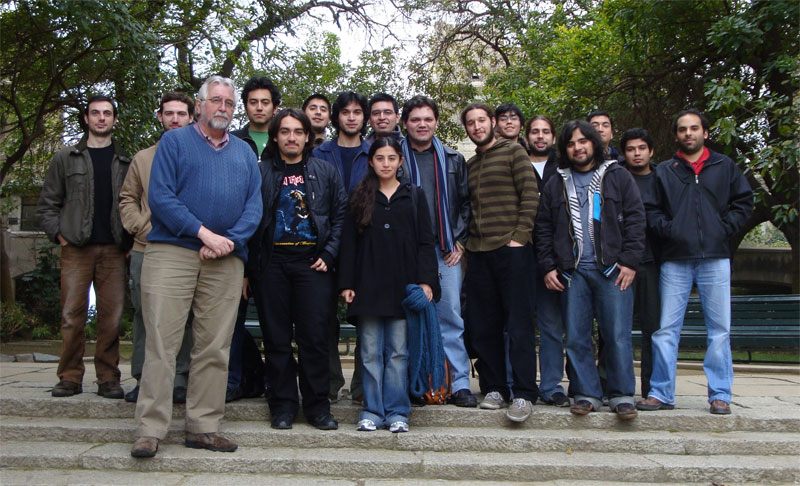
\includegraphics[width=0.8\textwidth]{images/alma-utfsm-1}\\\vspace{1cm}
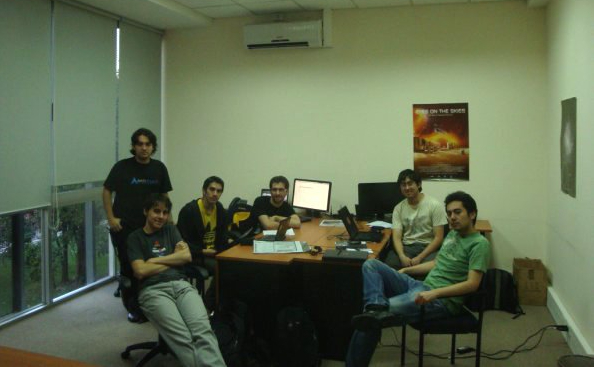
\includegraphics[width=0.8\textwidth]{images/alma-utfsm-2}\\
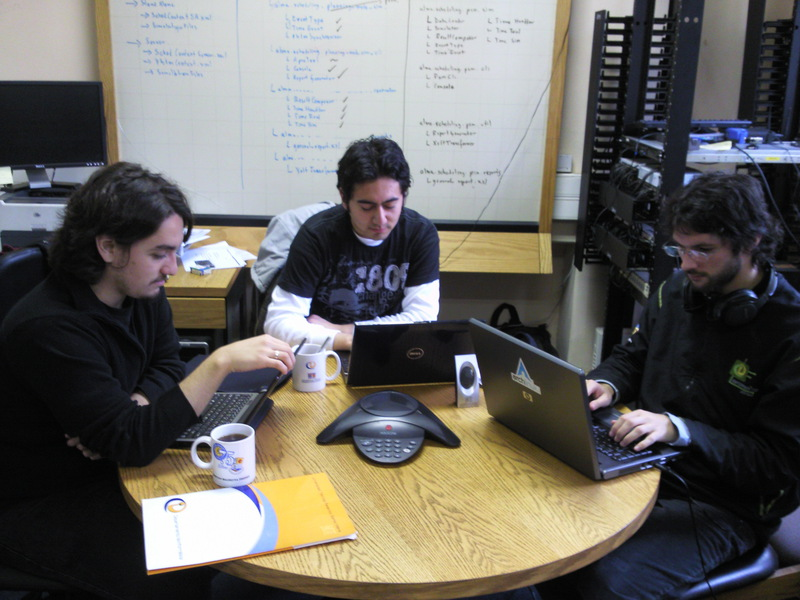
\includegraphics[width=0.8\textwidth]{images/lab_conference}\\\vspace{1cm}
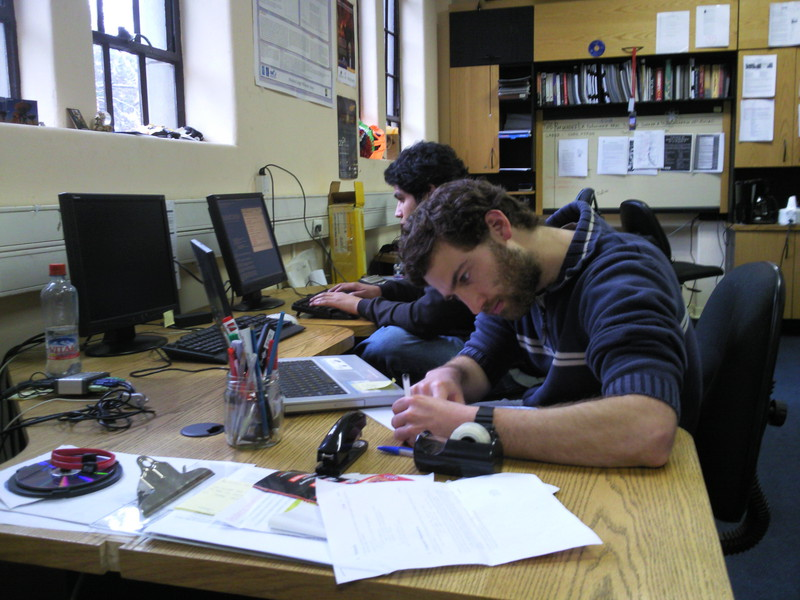
\includegraphics[width=0.8\textwidth]{images/lab_working}\\
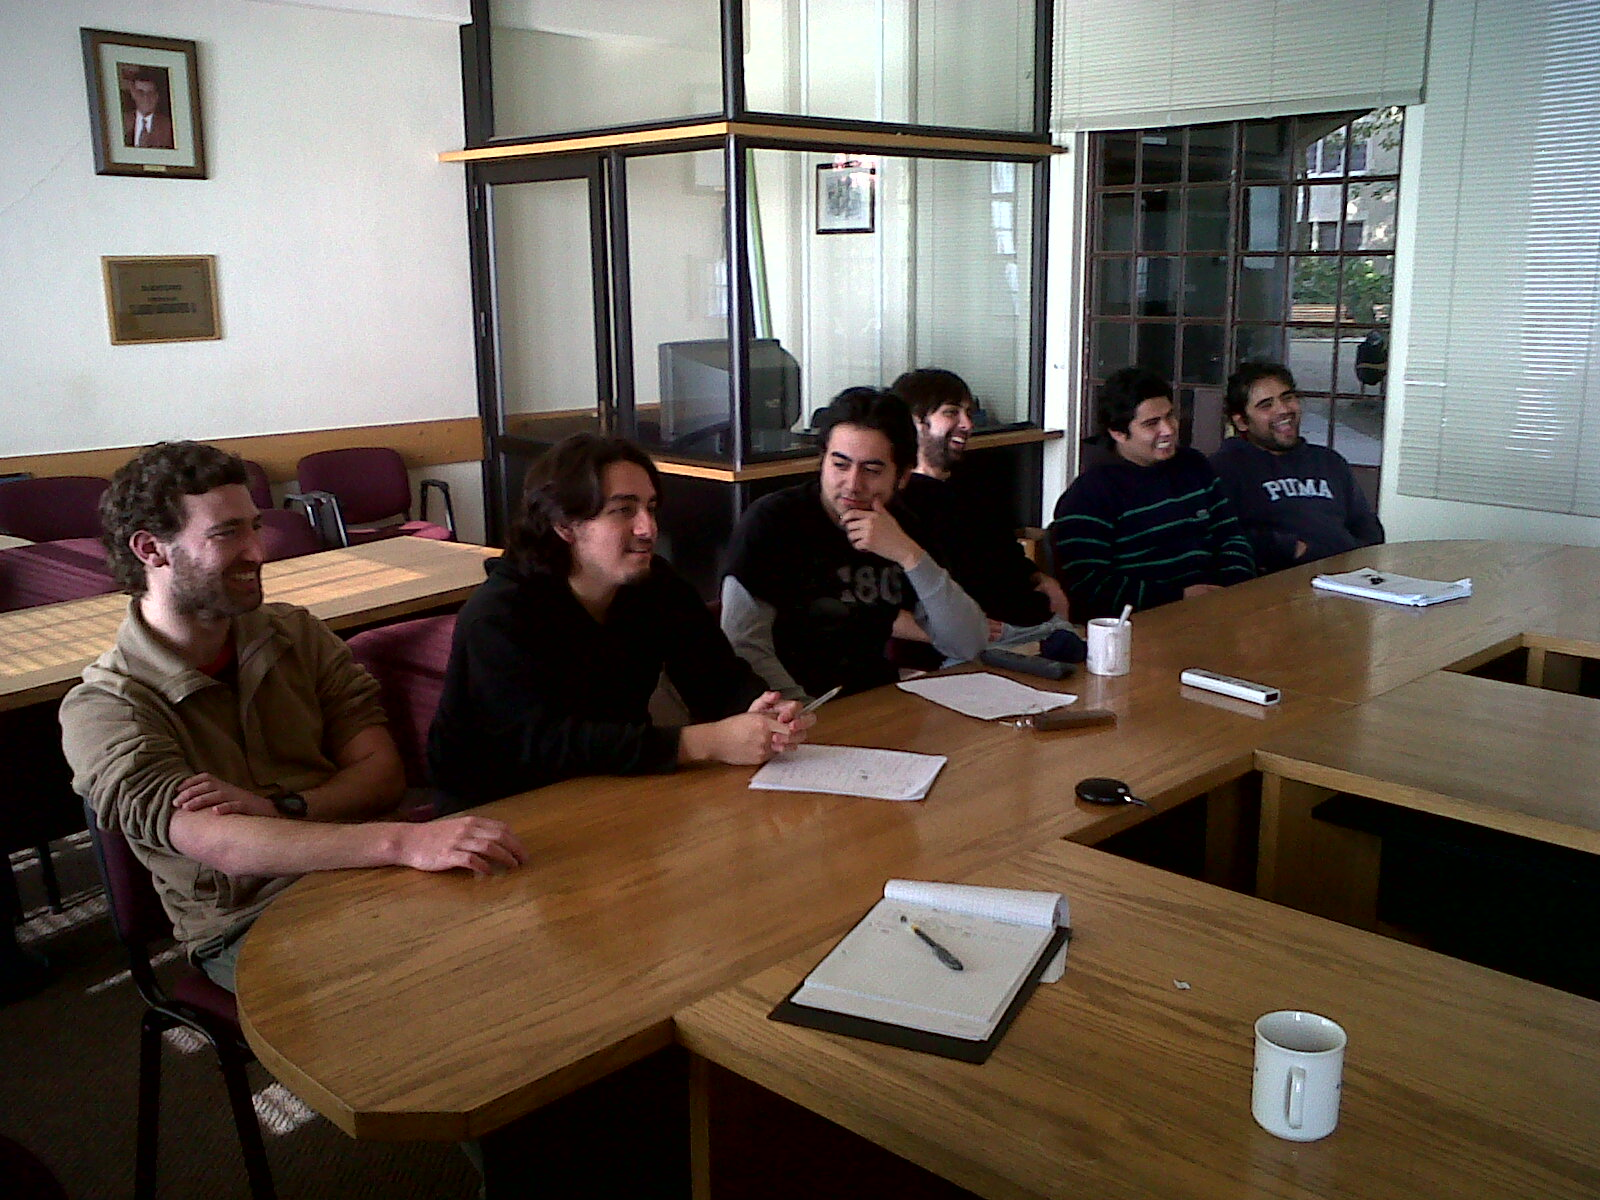
\includegraphics[width=0.8\textwidth]{images/leads1}\\\vspace{1cm}
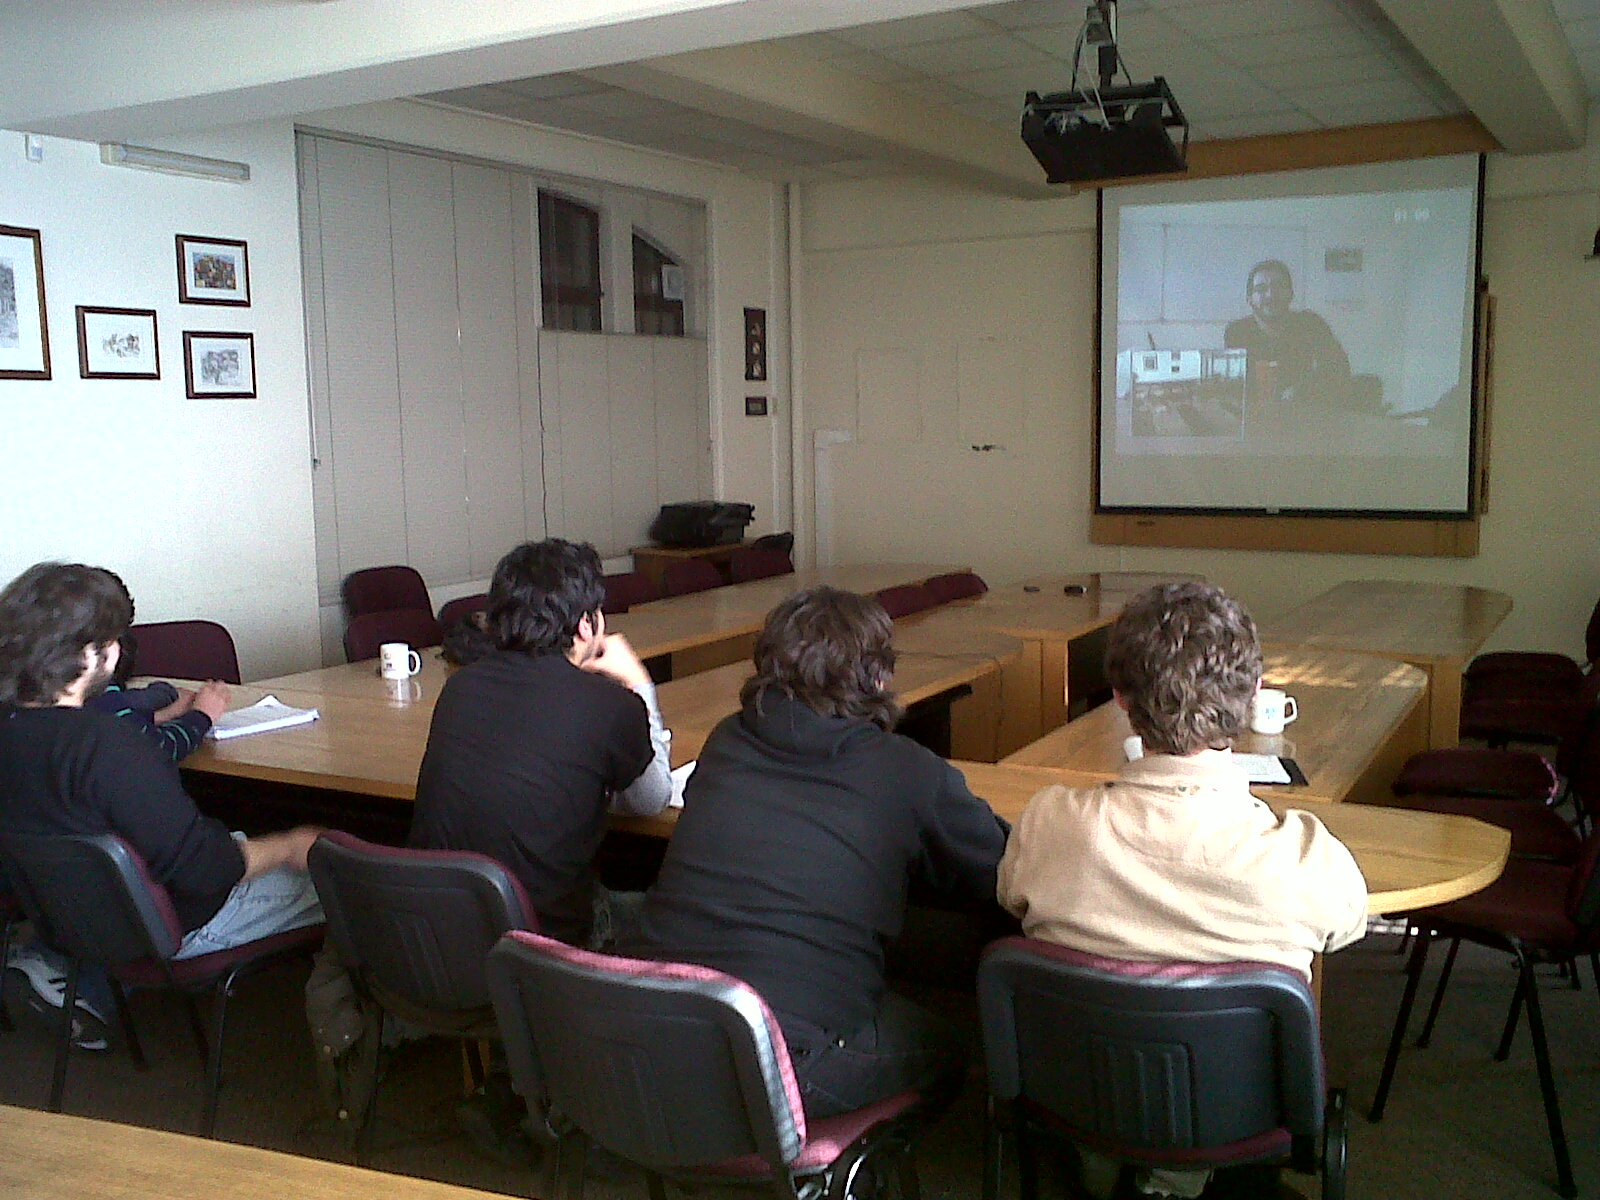
\includegraphics[width=0.8\textwidth]{images/leads2}
\end{center}
% CORRECCION &

\newpage
\subsection{Minutas de reuniones}
\subsubsubsection{ACS Weekly Meeting}
\begin{verbatim}
ACS Weekly Phone Meeting 
Date: Monday, 2010-04-12 

Attendees: 
ESO: Bogdan, Gianluca, Heiko, JosephSchwarz, 
NRAO: ArneGrimstrup, JorgeAvarias 
JSI: 
AOT: 
ALMA Chile: Ale 
UTFSM: GabrielZamora CristianMaureira 

Control contact number: +1-203-607-6471 (Passcode 203403#) 

General issues 

Alma has a promising candidate for a new board to replace the VMEs with 64 
bit architecture, to support more memory. Details from Thomas J. 
All module owners please fix their tests on 8.2 branch and HEAD. 

Ale Caproni 

Last week: 

CONTROL: Some issues with TotalPower testing, also due to STEs gotten messed up 
by other testers. 
The TP component has been changed to use the C++ API of the Bulk data libs, 
without reusing the IDL wrapper of the bulk data component. This works fine 
now, but still would like to discuss changes to the BD IDL for the long term. 
Will be at ESO early May. Things to be discussed should be added to Ale's 
Main.May2010 page.

Arne Grimstrup 

Last week: 

Continued investigation of COMP-3072 (with J. Avarias) 
problem still occurs with RHEL 5.4 version of CASA 
select is monitoring a bad file descriptor which triggers an exception 
in the TAO code. Telecon with UTFSM regarding future projects 
(with G. Chiozzi, H. Sommer, et. al.) Support 
Investigation of 64-bit test faults in NRI (H. Sommer)(with J. Avarias) 
Template method was invoking unsigned long version of getValue method 
that didn't exist Documentation for generated Python bindings (J. Kern) 
Questions regarding Python Binding Generator (J. Kern) 
Problem building ACS in INTROOT (J. Avarias) 

This week: 
Continue work on COMP-3072 
Continue work on COMP-830 

Bogdan Jeram 

Last week: 
Monday public holiday 
4 days of vacation 

Heiko Sommer 

Last week: 

Worked out HibernateDAL's usage of Archive's new archiveConfig.properties 
mechanism, together with Holger. 
Finalized 8.1 CVS logs and release notes. Pre-release of 9.0 VM. 
Discussions, e.g. TP with Ale and others 
Support, e.g. XSD validation, CDB performance fix, manager error messages, 
1 day leave 
Telecon with UTFSM about current projects 
quarterly report for ESO 

Helmut Tischer 

Last week: 
Vacation 

This week: 
COMP-2214 continuing 

Joe Schwarz 

Last week: 

Discussed problem of simultaneous use of SB by > 1 STE; change in 
lifecycle-handling needed 
Reviewed FP6 quarterly report from U. of Cambridge 
Worked on Total Power crash of Java container; suggested JNI 
debugging options for JVM runtime to Jeff and Ville, also removing
 native method invocation from class constructor (this didn't 
make any difference, however); got help from Roberto, who looked 
at logs and said he saw no bulk data issues 
Discussed CDR8 preparations w/Heiko 
Tried (and failed) to convince Brian to take Observation Control 
(not yet delivered) out of R7.1 
One day's leave 

This week: 
CDR8 preparation, ACS 9.0 planning 
Continue investigation of Total Power problem 
Return to classpath generation 

Jorge Avarias 

Last week: 

COMP-3749: ACS to introduce a new log level between DEBUG and TRACE 
Finished to make the last changes to the tests (Changed ACS_LOG_STDOUT 
from 2 to 1 new trace) 
All the tests affected by this are passing. 
Continued investigation of COMP-3072 (with A, Grimstrup) 
Fixed NRI ACS 64 bits building problems: 
The method unsigned long cdb::DAONode::getValue(char const*) 
was missing. probably some code is using unsigned long instead 
CORBA::ULong (in 32 bits they have the same length, in 64 they have not) 
Support: 
CONTROL/ACC/cppContainer crash (T. Powers) 
CONTROL/ACC/javaContainer crash, JVM is crashing with Seg. Fault 
(J. Kern, V. Suoranta) 
Problems building ACS in INTROOT (ACS is already built in ACSROOT) 
(S. Rankin) 


Matej Sekoranja 

Last week: 
HibernateDAL now skips loading all .dtd files, XMLSchema.xsd and xml.xsd so 
that Oracle's XMLTYPE checks don't get confused. 

This week: 
At CERN, but available for emergency ACS work. 

This week: 
TMCDB integration at the OSF 

UTFSM 

Last week: 

DDS Logging Service 
All the main goals are completed 
There are one pending task, write a "state of art" in this topic, for the paper 
accepted in the SPIE Meeting with people at ESO to define project objectives. 
Planning
Python support for BACI Properties 
ACS Code Generation 
ACS Windows Porting (Rodrigo and Heiko to integrate Java porting, Camillo and 
Gianluca to continue with C++ porting)
\end{verbatim}
\newpage
\subsubsubsection{OSF Coordination Meeting}

\begin{verbatim}
Date: Tue, 2010-05-18, 11:00 Chile, 9:00 Socorro, 17:00 Germany 
Attendees: 

ALMA-Chile: MatiasMora 
NRAO-Socorro: JorgeAvarias 
ESO-Garching: HeikoSommers 
UTFSM: GabrielZamora, TomasStaig, ArturoHoffstadt, CristianMaureira 
UCN: JaimePavlich 

Contact Info 
When: 11:00 Chile / 9:00 NM / 17:00 Germany 
Chile (toll free): 800532833 
International: +1 3032480281 
Access Code: 4676238 
Web Conferencing URL: http://net.globalcrossing.com/conferencing/ 

Agenda 
ALMA-CONICYT #31090034 (UTFSM) 
Projects 
ACS Windows Porting: The first version of the gcc-wrapper (gcc -> cl) is 
ready, we need to test with real examples to improve it. 
Code Generation: Luigi sent us a project proposal. Because Luigi was on
 vacations the last week, the meeting for this project is pending 
Alarms Configuration GUI: 
The project is ready, but there are some details with the redaction. 
Rules view that Tomas will fix in the week. 
Cristian Maureira and Tomas Staig will work on the documentation the 
next week. 
Official acceptance by ACS. 
Sampling System GUI: 
Juan Reyes and Cristian Maureira closed two of the three pending bugs, 
there are only one pending, that will be ready during the week. 
Official acceptance by ACS. 
ALMA-CONICYT #31080031 (AIA) 
Teams working on papers and on a new task about implementing TSP with 
their paper techniques 
HPC must to define the input framework and do some testing with TSP 
SebastianDuran and WalterFarina will be helping MatiasMora on what 
he needs for his thesis 
Second class this week Valpo. and next week Stgo. about advanced 
AI techniques 
Looking for possibilities of collaborations with MAIA-INRIA 
Summer Jobs 2010 
Pending reports! 
UCN Current Status 
Mini-ACS-Workshop from April 27th to May 10th. Funded by 
ALMA #31090026. 
Repository for UCN projects: http://goos-acs.googlecode.com 
gCCD status 
Implementing support for SBIG cameras 
Moving configuration to CDB 
gDome status 
gDome group are new students. After several intensive sessions 
they created the first version of the Dome component. 
Documentation: installation and system manuals. 
Misc 
ACS Scientific Linux distribution mirror repo here at UTFSM (ArturoHoffstadt).
\end{verbatim}
